\section{La Recherche Opérationnelle}
\subsection{Description et objectifs}
La Recherche Opérationnelle est définie comme étant la discipline des méthodes scientifiques utilisables pour élaborer de meilleures décisions~\cite{gamif-def}. Elle propose des modèles conceptuels permettant à des décideurs d'analyser des situations complexes et de faire rapidement les choix les plus efficaces. La Recherche Opérationnelle recouvre l'optimisation et l'aide multicritère à la décision. Elle permet de comprendre et modéliser un problème, proposer des méthodes de résolution et les tester, puis de les confronter à la réalité.\par
La Recherche Opérationnelle est notamment appliquée aux domaines de la production, du transport, des télécommunications, de l'aérospatial ou des réseaux informatiques. Elle permet d'apporter des améliorations à l'organisation, à la prise de décisions et des gains de temps et productivité.

\subsection{Enseignement}
Au sein de l'Université Paris-Nanterre, la Recherche Opérationnelle est enseignée de la même manière que les autres cours, c'est à dire en cours magistraux et séances de travaux dirigés/pratiques.\par
Les cours magistraux consistent en la dispense d’un enseignement majoritairement théorique par un enseignant à un large groupe d’apprenant. Ils ont pour but d'en transmettre les notions et points clés nécessaires à leur compréhension et application.\par
Les travaux dirigés et les travaux pratiques consistent en un enseignement plus souvent pratique de notions et connaissances à un groupe d’apprenants plus réduit. Ils ont pour but la réalisation d’exercices, qui peuvent ensuite être rendus à l'enseignant pour notation ou correction, ou simplement corrigé en groupe. Ceux-ci permettent ensuite à l’enseignant de compléter ou reprendre les enseignements théoriques au cas par cas avec les apprenants afin de valider l’acquisition des connaissances transmises lors des cours magistraux. 

\subsection{Évaluation des compétences}
Dès la rentrée 2019, l'enseignement de la Recherche Opérationnelle au sein de la MIAGE de l'Université Paris-Nanterre va se concentrer sur l'apprentissage et la validation de compétences clés. Actuellement, la matière est enseignée de manière linéaire, chapitre par chapitre, en réalisant divers exercices de mise en pratique des notions de cours tout au long de l'enseignement, puis validée par une évaluation finale couvrant l'ensemble de la matière. \par

Désormais, le cours sera articulé autour de notions clés. Ces notions sont définies par un nom décrivant de manière globale son objectif, par exemple "Optimiser en univers combinatoire". La notion est ensuite divisée en compétences à évaluer et valider. Celles-ci sont composées d'un verbe correspondant à l'action globale attendue (identifier, comparer, choisir, utiliser, etc.) puis de l'action précise qui vient compléter ce verbe ("les types de problèmes énumérables et leur complexité"). On obtient ainsi clairement les actions que l'étudiant doit être capable de réaliser pour considérer la compétence comme acquise. \par 

Afin de valider ces notions, les exercices d'application ont été revus. Chaque énoncé propose un problème et un contexte où celui-ci se pose et est suivi d'une zone de réponse prévue pour que l'étudiant y décrive son raisonnement et détaille sa réponse au problème. Chaque feuille d'exercice portera sur une des notions d'une compétence à valider, permettant de vérifier la compréhension et l'acquisition de cette compétence par l'étudiant. Ces exercices tout au long de l'enseignement seront comme actuellement accompagnés d'une évaluation de fin de parcours portant sur l'ensemble du cours de Recherche Opérationnelle. Cependant, il sera possible pour les élèves de savoir plus précisément quelles notions ont été saisies et lesquelles risquent de nécessiter plus de travail.

\section{Mise en place de la gamification}
\subsection{Mécaniques existantes et leurs transcriptions}
Afin de réaliser la gamification d'un enseignement, de nombreux outils sont à la disposition des enseignants. Ils doivent être adaptés à l'environnement d'application et peuvent prendre de nombreuses formes afin de correspondre au groupe qui en bénéficiera~\ref{fig:framework_gamif}. \par

\begin{figure}
    \centering
    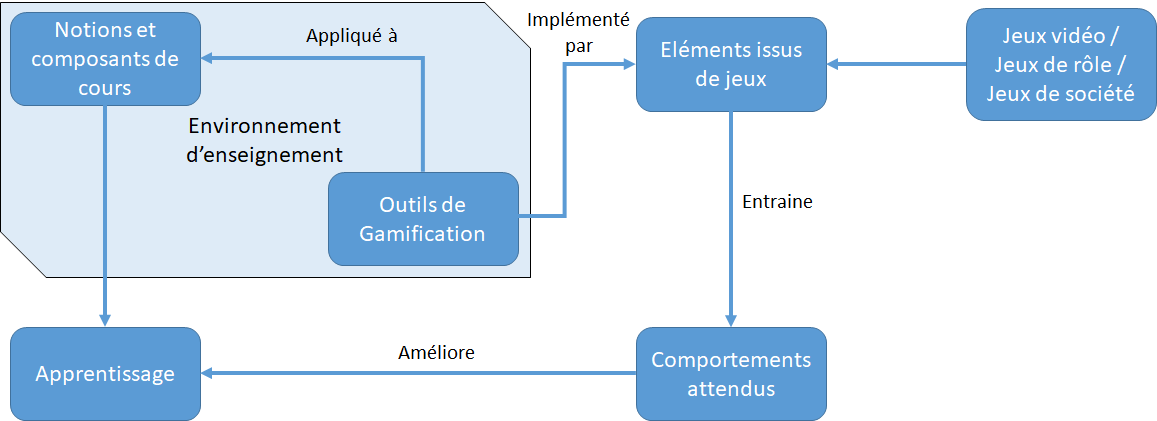
\includegraphics[width=\linewidth]{Images/Framework_Gamification_Education.png}
    \caption{Framework d'application, fonctionnement et résultats de la gamification à un contexte d'enseignement}
    \label{fig:framework_gamif}
\end{figure}

\subsubsection{Montée de niveau et gain d'expérience}
Outil classique et très fréquemment utilisé, la montée de niveau est simple à comprendre et expliquer aux participants : le niveau du joueur augmente d'un cran dès qu'un certain nombre de point d'expérience est acquis. On peut définir dans le cadre du jeu que le nombre de points requis est constant pour chaque montée de niveau, ou à l'inverse que chaque niveau atteint demande plus de points que le précédent. La deuxième option permet de rendre chaque montée plus gratifiante que les précédentes, tant que l'augmentation du nombre de points requis n'est pas disproportionnée ; si la montée de niveau devient trop laborieuse, on court le risque de démotiver les participants qui se contenteraient alors du niveau atteint jusqu'alors. De même, si augmentation il y a, elle doit suivre une logique et une formule déterminée afin que les montées de niveaux ne semble pas impossible sans une implication excessive dans le jeu. \par

Mettre en place un système de niveau dans un enseignement peut se faire de différentes manières. On peut par exemple définir que chaque participation en cours, que ce soit en répondant oralement ou en allant résoudre un exercice au tableau, fait gagner à l'étudiant un certain nombre de points. Les exercices à faire à la maison ou à rendre en fin de séance ainsi que les examens en rapporteraient également. A chaque niveau gagné, on pourrait remettre une petite récompense à l'élève, liée ou non au cours, physique ou virtuelle. La récompense n'aurait pas besoin d'être conséquente mais sa simple existence permettrait de donner un but à cette montée. Une seconde manière de faire serait simplement que chaque grande notion de cours comprise et validée par une évaluation fasse monter l'étudiant d'un niveau directement. Le niveau devient alors une mesure de la compréhension globale de l'enseignement, bien que cela puisse décourager ceux qui auraient quelques niveaux de retard sur le reste de leur classe. Pour contrer cela, insister sur les notions incomprises auprès des concernés pour les ramener au même niveau que les autres, aussi bien en terme de connaissance que de jeu, semble une bonne solution. Un exercice supplémentaire à réaliser chez soi et donnant une quantité légèrement moindre de point  permettrai de compenser ce retard, de permettre à l'étudiant de s'entraîner et de ne pas sortir du jeu. 

\subsubsection{Succès et badges}
Un autre outil phare du jeu vidéo relativement simple à appliquer est le système de succès ("Achievements") et de badges. La première apparition de ce système dans le jeu vidéo date de 1982 où Activision envoyait aux joueurs leur fournissant une photo de leur meilleur score dans un de leur jeu un patch vestimentaire exclusif. Plusieurs jeux vidéos ont par la suite inclus des contenus cachés disponibles en réalisant des actions précises, comme le jeu E-Motion sorti sur Amiga en 1990, ou des titres et badges affichés sur le profil du joueur et visibles même en dehors du jeu, comme le jeu de rôle massivement multijoueur en ligne World of Warcraft. Le système de succès et de badge a réellement commencé à se démocartiser grace à la console de jeu XBox 360 de Microsoft où une majeure partie des jeux proposaient des succès plus ou moins recherchés et complets, allant de simplement terminer une partie du jeu à réaliser des actions longues et complexes durant sa partie. \par

Les succès sont une composante de gratification assez simple à appliquer durant un enseignement. On peut imaginer que chaque travail pratique réalisé, rendu et réussi, ou chaque grande notion de cours validée par une évaluation, permette l'obtention d'une badge (physique ou numérique) afin de témoigner de la réussite de l'étudiant. On peut également lier l'attribution de badges à la montée de niveau de l'élève comme précédemment évoqué, en guise de récompense pour avoir atteint un niveau prédéfini. Dans le cadre d'une récompense physique, comme un badge à imprimer, un sticker ou autre chose, l'enseignant devrait être celui qui le distribue (et si besoin le fabrique, comme dans le cas du badge). Cela permettrait un meilleur arbitrage et contrôle de leur distribution et répartition, en évitant que certains participants trichent et décide de réaliser des copies qu'ils distribueraient, diminuant la valeur de cette récompense et encourageant la triche.

\subsubsection{Classement des participants}
Majoritairement utilisé au début de l'histoire des jeux vidéos, le classement des meilleurs scores (associés ou non à un nom ou pseudonyme) est une autre forme de gratification applicable à l'enseignement. Historiquement très utilisé dans les bornes d'arcades et les premiers systèmes de jeu (notamment les micro-ordinateurs et les consoles "8 bits"), classer les participants selon leurs performances peut permettre de les motiver à mieux faire et introduire un peu de compétition et de challenge dans le cadre du cours. Il est toutefois à noter qu'un classement nominatif des étudiants pourrait décourager deux des quatre profils de joueurs, à savoir les "Explorers" et les "Socializers"~\ref{fig:bartle}. Les premiers ne cherchent pas à se comparer aux autres mais surtout à découvrir tout ce que le cours peut leur apporter ; les seconds cherchent avant tout à tisser des relations avec leurs autres joueurs et à profiter d'un esprit d'équipe. \par

Un classement général anonyme avec la possibilité d'obtenir du professeur son classement personnel par rapport au reste de la classe semble un bon compromis. On motive à la fois les "Killers" et les "Achievers" à se dépasser en leur donnant une échelle à laquelle monter et se comparer, sans afficher devant tout le groupe le niveau de chacun. On peut également imaginer que le classement personnel donné par l'enseignant ne serait pas le rang exact de l'étudiant mais par exemple dans quel quart du classement se situe l'élève. Cela fournirait également un bon outil au professeur pour savoir quel étudiant semble en difficulté ou en retard dans le jeu, lui permettant d'adapter au besoin le reste du cours.

\subsubsection{Jeu de rôle et travail d'équipe}
Comme son nom l'indique, un jeu de rôle est un genre de jeu de plateau ou de jeu vidéo où le joueur incarne un ou plusieurs personnages au sein d'un monde imaginaire plus ou moins détaillé et aux règles prédéfinies. Les plus connus et populaires inclus entre autre le jeu de rôle papier "Dungeons and Dragons" et ses déclinaisons vidéoludiques ou les séries de jeux vidéos "Pokémon" ou "The Elder Scrolls". Dans le cadre de la gamification, la mise en place d'un jeu de rôle consiste à recréer une situation réaliste où le système gamifié est mis en application. Par exemple, lors d'un cours de marketing, un élève jouera le rôle d'un vendeur et l'enseignant celui du client, afin de mettre en pratique dans un contexte fictif et ludique les notions vues en cours. Le fait d'impliquer les élèves dans l'enseignement qui leur est prodigué via un jeu de rôle montre une amélioration des résultats, d'implication et du ressenti positif des étudiants vis à vis ce celui-ci~\cite{role-playing-educ}. \par

Le travail en équipe quant à lui permet de créer un contact et une sociabilisation des participants. Afin de résoudre un but commun, ceux-ci sont dans l'obligation de coopérer, de mettre en commun leur idées et talents, et de réaliser un objectif commun où chacun est indispensable au bon fonctionnement de l'entité. En plus de satisfaire les "Socializers", il permet également aux "Explorers" de découvrir d'autres points de vue et méthodes de résolutions. En entretenant une compétition entre équipe, il est également possible de motiver davantage les "Killers" et "Achievers", permettant donc une amélioration globale de l'implication des participants. Sauf cas où certains participants sont plutôt individualistes ou travaillent mieux seuls, les travaux de groupe sont une bonne solution pour garder l'ensemble du public cible impliqué dans le jeu, et par conséquent le système gamifié. \par

Pour gamifier un cours de d'informatique, il serait possible de concevoir des exercices de mise en situation précis et concrets, où des équipes serait chacune mise face à un problème concret à résoudre, où l'enseignant pourrait jouer le rôle d'un client ou simplement de maître du jeu. Chaque membre de l'équipe détiendrait des informations différentes concernant le problème à résoudre, forçant la mise en commun et la communication au sein de l'équipe afin de comprendre et mettre en relation ces données. Chaque équipe aurait pour but de résoudre le plus vite possible de manière correcte son problème avant de rendre sa solution à l'enseignant qui se chargera de l'évaluer. Pour augmenter le défi il serait possible de limiter dans le temps la résolution de l'exercice, pour forcer la communication à être la plus efficace et claire possible. A la fin du temps imparti, chaque équipe changerait de sujet à résoudre, de composition ou les deux, pour voir si une autre configuration ou un autre objectif fonctionne mieux avec eux, et pour mettre en pratique un autre aspect de l'enseignement. Enfin, la réalisation d'un classement des équipes avec un badge exclusif ou un gain d'expérience plus important pour ses membres en fin d'exercice permettrait de mettre en pratique toutes les mécaniques précédemment abordées.

\subsection{Évaluer la réussite des étudiants}
L'évaluation actuelle des étudiants est réalisée tout au long du module par des exercices et en fin de module par un contrôle terminal. Les exercices corrigés pendant les séances avec l'enseignant et les résultats de chacun sont échangés, expliqués ou débattus. Une ou deux évaluations notées de mi-parcours ont lieu, complétées par l'évaluation finale de fin de module. \par 

Désormais, ce modèle sera complété par une évaluation par l'enseignant des notions au fur et à mesure du cours. En fonction des résultats aux exercices proposés dans le cadre du module, l'enseignant déterminera si les étudiants ont validé celles-ci ou non et pourra proposer des exercices complémentaires à effectuer pour s'améliorer à ceux qui auraient échoués. Les notions ne sont pas évaluées directement par un exercice précis, mais plutôt par croisement des différents résultats des étudiants. Les activités proposées en cours (voir~\nameref{appendix-activity-or}) sont constituées de plusieurs exercices, et sont pensées pour être aussi bien réalisées en auto-évaluation chez soi que dans le cadre des travaux dirigés. \par

\subsubsection{Activités et exercices}
La première activité prévue a pour but d'apprendre l'identification des problématiques de Recherche Opérationnelle. Les étudiants devront, pour une série de photographies présentant un cas d'application, identifier un maximum de problématiques à résoudre afin de veiller au bon fonctionnement du système. Par exemple, à quels problèmes de logistiques est confronté un aéroport ou le réseau ferré français. L'exercice consiste à donner au moins dix problématiques par cas sous forme de mots-clés ("bagages", "passagers", "parking", etc.). Dans le cas de l'auto-évaluation, une liste de mots-clés possibles sera fournie à l'étudiant une fois son exercice réalisé afin qu'il compare ses résultats. Dans le cas d'une réalisation classique en cours, l'enseignant discute les résultats qu'il avait sélectionné et ceux trouvés par les étudiants. On considérera que l'activité est réussie et validée si, pour chaque cas, au moins 80\% des réponses étaient dans la liste de l'enseignant, puis si 80\% des cas ont rempli cette condition. \par

La seconde activité valide la compréhension des graphes et de leurs propriétés et représentation. Les exercices consistent ici à déterminer de manière graphique si un graphe répond à tel ou tel critère ou certaines de ses propriétés (s'il est orienté ou non, ou son nombre de sommets par exemple), de donner leur représentation graphique ou encore de généraliser un résultat. L'évaluation est ici plus traditionnelle, chaque réponse est juste ou erronée et correspond à une question. Afin de considérer l'activité comme réussi et validée, au moins 80\% de bonnes réponses sont attendues, et aucun exercice ne doit avoir été ignoré complètement. On attend de l'étudiant qu'à défaut d'avoir la bonne réponse, il puisse au moins fournir un raisonnement et une ébauche de solution. \par

Les deux activités suivantes sont complémentaires et visent à résoudre des problèmes par des graphes et à effectuer diverses démonstrations. Ces exercices demandent de réaliser des graphes répondant aux énoncés, de montrer des propriétés des graphes et d'en déduire des résultats ou encore d'appliquer des algorithmes  à des graphes donnés. Leur validation demande 80\% de bonnes réponses et que les exercices soient au moins en parti réalisés, de la même manière que la seconde activité. \par

Une activité d'entraînement réalisable à distance sera proposable afin que les étudiants puissent réviser leurs notions tout en réalisant un jeu. L'exercice n'aura pas de limite de temps ou de nombre de réalisations. Les étudiants seront soumis à des questions ou à des affirmations accompagnées ou non d'un graphe ou d'une représentation graphique. Pour chacune d'elles, plusieurs choix de réponses seront disponibles, sous la forme d'une réponse par vrai ou faux, de plusieurs réponses mutuellement exclusives ou de réponses à choix multiples admettant plusieurs réponses. Le but de l'exercice est de vaincre un "boss de fin de niveau" possédant un nombre de point de vie, chaque bonne réponse lui faisant perdre un montant défini à l'avance. En revanche, l'étudiant possède lui aussi un nombre de point de vie et chaque mauvaise réponse lui faisant perdre un montant également. Le but de l'exercice est de vaincre le "boss" sans perdre tous ses propres points. Un classement personnel sera ensuite montré à l'étudiant avec ses meilleurs résultats, c'est à dire son nombre de bonnes réponses et son nombre de points de vie restant à la fin de l'exercice. Un classement global de sa promotion pourrait également lui être proposé. Afin d'encourager davantage à continuer à jouer, les mauvaises réponses afficheront une explication de la réponse attendue. \par

Une dernière activité, réalisable par groupes de trois ou quatre étudiants, est également envisageable et proposerait un entraînement sur des exercices plus poussés. Trois sujets d'exercice sont proposés successivement à chaque groupe : réalisation de graphes, démonstrations de propriétés et analyse de graphes. Ces sujets sont complémentaires aux activités précédentes en poussant leur difficulté plus loin afin que le travail de groupe soit nécessaire à leur réalisation. Chaque résolution de sujet est chronométrée, puis chaque groupe rend sa copie et passe au sujet suivant, avant de répéter le processus une dernière fois. Une fois les trois copies par groupe rendues, les exercices sont corrigés puis notés par l'enseignant en présence des élèves. Les groupes seront ensuite classés selon leurs résultats. La bonne communication au sein du groupe et la participation de chacun seront les éléments clés de la réalisation de l'activité.

\subsubsection{Modalités d'évaluation}
Le taux de bonnes réponses de 80\% a été choisi afin de s'assurer une compréhension globale des notions du cours et encourager les étudiants à les réviser et les approfondir pour les repasser en auto-évaluation par la suite si le taux n'est pas atteint. Il est tout à fait possible de moduler ce taux en y appliquant une variable $x$ d'une valeur comprise dans l'intervalle $[0,8\;;1,2]$. Cette variable permet de moduler le taux de 64\% à 96\% et ainsi d'adapter l'évaluation aux résultats des étudiants. \par

En cas d'exercice ou d'activité réalisée en groupes, par exemple l'identification de problématiques ou la compréhension de graphes et de leurs propriétés, la notation ne change pas mais la consigne peut varier légèrement. Pour encourager l'échange entre les étudiants et la confrontation de pistes et d'idées diverses, la difficulté de l'exercice devrait être supérieure pour demander une réflexion plus complète. Ce type de travaux ne rentre pas complètement dans l'évaluation des acquis mais davantage dans la stimulation de la réflexion et la compréhension plus profonde des notions abordées par le cours. L'incorporation d'une composante de jeu de rôle peut renforcer le travail par groupe en mettant en situation les étudiants et en leur demandant l'adoption d'un point de vue de réflexion différent. 

\subsection{Gamification des activités et exercices}
La gamification du cours de Recherche Opérationnelle se fera selon deux axes principaux : un système de gain d'expérience et de montée de niveau, et un système de badges pour récompenser les étudiants. \par

Les étudiants commenceront le module avec un niveau d'expérience de 1 et gagneront un niveau tous les 250 points d'expérience acquis. Lors de la réalisation d'une activité, chaque exercice validé rapportera 50 points, qu'ils aient été effectué durant la séance de travaux dirigé ou en auto évaluation. Si l'activité est validée à 100\%, c'est à dire si chaque exercice de l'activité est réussi à $x$ x 80\%, un bonus de 100 points est attribué à l'étudiant. Un étudiant absent sans justification lors de la séance mais réalisant en auto-évaluation une activité par la suite marquera la moitié des points qu'elle devrait lui rapporter, mais aura tout de même accès au bonus. \par

Ces valeurs ont été choisies pour que l'élève monte de niveau approximativement à chaque activité, dans le but de le motiver à réaliser au mieux les exercices. Il est bien sûr possible d'appliquer à ces gains une variable $y$ comprise dans l'intervalle $[0,5\;;1,5]$ en fonction du taux de bonnes réponses demandées. Par exemple, pour une valeur de $x$ basse, on pourra baisser en conséquence $y$ pour signifier que l'exercice était simple, et inversement avec une valeur de $x$ plus élevée. \par

L'attribution de badges pourra se faire aussi bien pour récompenser une montée de niveau ou une réussite dans le cadre de l'enseignement. Ces badges peuvent aussi bien être virtuels et accessible via un service à déterminer, il est possible de les imprimer et de les distribuer. Si récompenser chaque montée de niveau risque de de diminuer l'impact positif de la récompense, une attribution à chaque niveau pair atteint permet une récompense rapide (le niveau de départ étant fixé à un), puis semi-régulière par la suite afin de toujours récompenser les efforts. Un badge peut être donné également quand une activité est validée à 100\%, voire quand tous les exercices de l'activité sont eux même validés et justes à 100\%. Dans le cas d'un exercice par groupe, un badge peut être attribué à l'équipe ayant réalisée le meilleur score ou ayant réalisé l'exercice le plus rapidement avec le moins d'erreurs, motivant à la fois le travail de chacun et la collaboration des membres. \par

Il serait également possible de réaliser un classement par niveau des étudiants afin que chacun puisse voir où il se situe par rapport à sa promotion. Cependant,  afin d'éviter le développement d'une compétition, la démotivation ou le surmenage~\cite{gamif-educ}, il serait judicieux de proposer un classement sur la base du volontariat s'il n'est pas anonyme. Ainsi, les plus compétitifs pourraient se comparer et chercher à faire mieux que les autres, tandis que les autres pourraient profiter des autres aspects de la gamification sans pression. Le niveau final atteint de chaque étudiant, une fois comparé par l'enseignant au reste de la promotion, pourrais également constituer une forme de note de contrôle continu ; un niveau élevé reflète une bonne compréhension et application des notions vues en cours.

\subsection{Rôle de l'enseignant}
La simple mise en place de ces activités seules ne permettra pas d'améliorer suffisamment l'apprentissage et l'engagement des étudiants. L'enseignant a un rôle actif à jouer dans la forme, l'évolution et la réalisation de son enseignement par ses exercices ses retours. La mise en place de "Techniques de Rétroaction en Classe" (ou TRC)~\cite{gamif-CATs}, ou "Classroom Assessment Techniques" (ou CATs) en anglais, lors des cours peut accompagner cette gamification afin de la réorienter, la faire évoluer en fonction des retours des étudiants. Les TRC permettent aux étudiants d'obtenir des informations sur leur avancement dans le cours, à quel point ils ont atteint ou non les objectifs, et d'avoir ainsi un retour en temps réel et objectif de la part de leur enseignant. Ces exercices d'une durée de cinq à vingt minutes en général donnent également à l'enseignant une bonne idée du niveau général du groupe d'apprenant concerné. \par

Les TRC sont des exercices centrés sur l'amélioration de l'apprentissage, aussi bien du coté des élèves que de l'enseignant. Ce dernier les met en œuvre sur un certain nombre de séances planifiées en amont, les adapte selon les résultats et le niveau des élèves et selon ses méthodes, et fournit aux étudiants un retour sur leurs compétences et leurs savoirs acquis. Les étudiants peuvent en retour améliorer leurs stratégies d'apprentissage en fonction de leurs résultats, en sachant que ces exercices anonymes et non notés sont un entraînement régulier. \par

Pour M. Daele~\cite{gamif-CATs}, les TRC sont basés sur sept présupposés issus de la recherche sur la pédagogie : 
\begin{itemize}
    \item "La qualité de l’apprentissage des étudiants dépend en grande partie de la qualité de l’enseignement
    \item Pour accroître leur efficacité, les enseignants devraient définir des objectifs pédagogiques puis fournir du feedback aux étudiants à propos de la façon dont ils sont en train de les atteindre
    \item Pour améliorer leur apprentissage, les étudiants ont besoin de recevoir un feedback approprié, rapide et régulier mais ils doivent aussi apprendre à évaluer eux-mêmes leur propre apprentissage
    \item Le type d’évaluation des enseignements qui permet le plus d’améliorer l’enseignement est celui qui correspond aux problèmes et aux questions que l’enseignant se pose à lui-même, ce qui veut simplement dire que le mieux est que l’enseignant puisse interagir directement avec les étudiants à ce sujet
    \item Le défi intellectuel et systématique constitue un moteur important de motivation, de développement et d’innovation chez les étudiants, et l’évaluation formative en classe peut y contribuer
    \item Les TRC ne demandent pas une formation particulière et elles peuvent être mises en place en classe par des enseignants de toutes les disciplines
    \item En collaborant avec des collègues et en impliquant activement les étudiants dans les TRC, les enseignants peuvent développer leurs compétences et leur satisfaction à enseigner"
\end{itemize}
\par 

Dans le cadre du cours de Recherche Opérationnelle, on peut imaginer qu'à partir de la deuxième séance, cinq minutes soient accordées à la fin du cours afin que les étudiants répondent à quelques questions simples sur des notions du cours précédent et à une ou deux questions sur une notion abordée le jour même. En complément, cinq à dix minutes en début de cours à partir de la séance suivant seraient utilisées afin d'analyser les résultats de la promotion et de discuter des points mal compris et de faire le point sur le niveau global des apprenants. L'enseignant pourra également fournir des conseils sur quelle notion retravailler en priorité ou des méthodes afin de mieux apprendre le contenu posant problème. Ces exercices placent l'enseignant dans un rôle de mentor vis-à-vis des élèves, qui additionné à la gamification des activités, lui permettront de mieux encadrer, encourager et guider la promotion pendant toute la durée du module.

\subsection{Hypothèse sur l'efficacité de la gamification}
Lors de l'année scolaire 2018-2019, l'enseignement de Recherche Opérationnel regroupait un total de cinquante-sept étudiants (voir \nameref{appendix-notes-or}). De ces résultats, nous pouvons en déduire divers taux qui serviront à vérifier l'efficacité de la gamification. Le taux de réussite de la promotion avant rattrapages et en incluant les absents est de 73,68\%. Quatre des étudiants de la promotion n'ont pas assisté au module ou à ses évaluations, soit un taux de 7,02\% des inscrit. En les excluant de nos observations, le taux de réussite de la promotion passe à 71,70\%. On observe une répartition des notes relativement équilibrée~\ref{tab:OR_notes_stats} avec un premier quartile à 9,7, un troisième quartile à 14,8 et un indice de dispersion de 15,6. La promotion a donc globalement validé, malgré des notes allant dans les deux extrêmes~\ref{fig:OR_notes_repart}. \par

\begin{table}
    \begin{center}
        \begin{tabular}{|c|c|c|}
        \hline
        \textbf{1er quartile} & \textbf{Médiane} & \textbf{3ème quartile} \\ \hline
        9,7                   & 11,5             & 14,8                   \\ \hline
        \end{tabular}
        \label{tab:OR_notes_stats}
        \caption{Informations statistiques sur les notes de Recherche Opérationnelle de la promotion 2018-2019 en Licence 3 à l'Université Paris-Nanterre}
    \end{center}
\end{table}

\begin{figure}
    \centering
    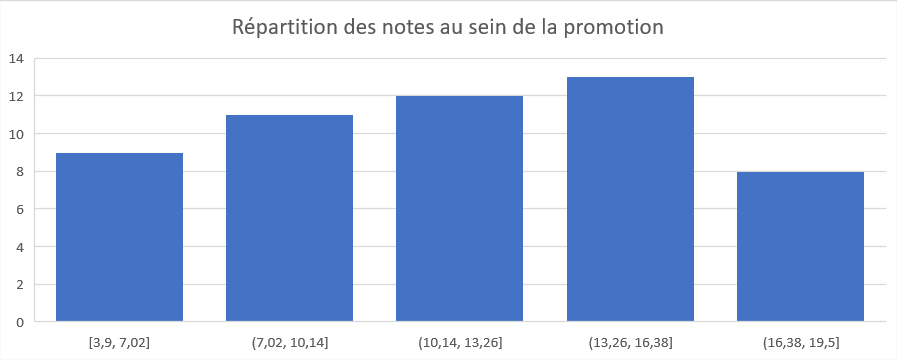
\includegraphics[width=\linewidth]{Images/Repartition_notes_RO.png}
    \caption{Répartition des notes de Recherche Opérationnelle de la promotion 2018-2019 en Licence 3 à l'Université Paris-Nanterre}
    \label{fig:OR_notes_repart}
\end{figure}


Notre hypothèse sur l'efficacité de la gamification, d'après les études réalisées~\cite{gamif-educ}, est que l'on devrait observer un taux de réussite au moins équivalent et une augmentation de la valeur des quartiles et de la note médiane. Le taux de présence devrait quand à lui baisser légèrement, tout comme l'indice de dispersion qui devrait diminuer.

\subsection{Évaluer l'efficacité de la gamification}
Afin de vérifier au mieux notre hypothèse, il nous faut pouvoir comparer les résultats attendus et obtenus à la fois du cours sans gamification et avec. Pour considérer que sa mise en application a amélioré la réussite des étudiants, la réussite globale du groupe doit avoir augmenté, mais l'écart entre les meilleurs résultats et les moins bons ne doit pas avoir augmenté pour autant. Dans le cas où cet écart se creuserait, la réussite de la gamification ne saurait être validée ; si les meilleurs le deviennent encore plus mais que les élèves en difficulté ne s'améliorent pas, la méthode n'est pas la bonne et n'a servi qu'à accentuer les différences entre les étudiants. \par

Les participants à l'expérience seront répartis dans un groupe témoin et un groupe de test. L'échantillonnage sera limité par la taille des promotions et risque de ne pas être significatif. En partant du postulat que chaque promotion fait une trentaine d'étudiants (en incluant les élèves en MIASHS parcours MIAGE et parcours Mathématiques) et qu'il y a deux promotions chaque année (formation initiale et formation en alternance), on peut imaginer deux moyens de comparer les résultats. \par

En incluant les deux promotions d'étudiants dans l'expérience, on obtient un échantillon de taille $n = 60$ environ, variant légèrement selon le nombre d'étudiants de chaque parcours\footnote{$n$ pourra être plus petit certaines années, selon le nombre d'étudiants dans les promotions, les abandons et les absents. On considérera ici $n$ comme étant à sa valeur prévue et optimale.}. Cet échantillon, bien que réduit, permet d'être relativement significatif tout de même. Il permet de comparer deux environnements et profils d'étudiants différents et d'adapter nos variables $x$ et $y$ précédemment évoquées de manière plus précise tout au loin de l'enseignement aux deux groupes. On peut ensuite réaliser l'expérience de deux manières. On peut pendant une année dispenser l'enseignement classique aux deux promotions qui serviront de groupe témoin global à $n = 60$ individus, puis lors de l'année suivante, mettre en place l'enseignement gamifié sur le groupe test, composé de la même manière de $n$ individus. On peut également lors d'une première année dispenser à une des promotions l'enseignement traditionnel et à l'autre l'enseignement gamifié, formant ainsi un groupe témoin et un groupe de test de $n = 30$ individus chacun, puis répéter le même procédé en inversant quel groupe reçoit quel enseignement une deuxième année. La deuxième méthode permet de prendre en compte l'éventuelle différence de niveau et/ou de comportement d'une promotion annuelle à l'autre. \par